\documentclass[10pt,a4paper]{article}

% Reproducible PDF metadata for a fixed TeX toolchain.
\pdfinfoomitdate=1
\pdftrailerid{}
\pdfsuppressptexinfo=15

\usepackage[T1]{fontenc}
\usepackage[utf8]{inputenc}
\usepackage{lmodern}
\usepackage{microtype}
\usepackage[a4paper,margin=23mm]{geometry}
\usepackage{amsmath,amssymb}
\usepackage{booktabs,tabularx,array,longtable}
\usepackage{seqsplit}
\usepackage{enumitem}
\usepackage{xcolor}
\usepackage{hyperref}
\usepackage{fancyhdr}
\usepackage{tikz}
\usetikzlibrary{arrows.meta,positioning,shapes.geometric,fit,calc}

\definecolor{navy}{HTML}{17324D}
\definecolor{teal}{HTML}{1B728C}
\definecolor{soft}{HTML}{F1F5F7}
\definecolor{warn}{HTML}{8A4B08}
\hypersetup{
  colorlinks=true,
  linkcolor=navy,
  citecolor=teal,
  urlcolor=teal,
  pdftitle={A Falsifiable Study of Siamese Embedding Compression for Face Verification},
  pdfauthor={Guillaume Harbonnier},
  pdfsubject={Corrected uncertainty analysis and closure of the initial 512D to 128D experiment},
  pdfkeywords={metric learning, face verification, face identification, embedding compression, PCA, random projection, non-inferiority, subject bootstrap, reproducibility}
}
\setlength{\parindent}{0pt}
\setlength{\parskip}{5pt}
\setlength{\emergencystretch}{1.5em}
\setlist[itemize,enumerate]{nosep,leftmargin=*}
\pagestyle{fancy}
\fancyhf{}
\fancyhead[L]{Siamese Embedding Compression v0.2.3}
\fancyhead[R]{Corrected initial experiment report}
\fancyfoot[C]{\thepage}
\renewcommand{\headrulewidth}{0.4pt}
\fancypagestyle{plain}{\fancyhf{}\fancyfoot[C]{\thepage}\renewcommand{\headrulewidth}{0pt}}

\newcommand{\fnmr}{\mathrm{FNMR}}
\newcommand{\fmr}{\mathrm{FMR}}
\newcommand{\DeltaFNMR}{\Delta_{\fnmr}}
\newcommand{\code}[1]{\texttt{#1}}

\title{\textbf{A Falsifiable Study of Siamese Embedding Compression for Face Verification}\\[5pt]
\large Corrected uncertainty, negative evidence, and a progressive research design}
\author{Guillaume Harbonnier\\
\small Independent exploratory research\\
\small \url{https://github.com/gharbonnier78/siamese-embedding-compression-lab}}
\date{Version 0.2.3 --- August 2026}

\begin{document}
\maketitle
\thispagestyle{empty}

\begin{center}
\fcolorbox{warn}{soft}{\parbox{0.92\linewidth}{\textbf{Scope.}
This manuscript reports a bounded research experiment on embedding compression. It is not
an industrial biometric validation, not a product qualification, and not evidence of
regulatory conformity. The source extractor is ImageNet ResNet-18 and the benchmark is
Labeled Faces in the Wild (LFW); both limit the inference domain.}}
\end{center}

\begin{abstract}
Reducing face-template dimension can lower storage and comparison cost, but a smaller vector
is useful only if decision-relevant biometric performance is retained. This paper turns a
pedagogical Siamese-network idea into a falsifiable experiment comparing four routes applied
to the same frozen 512-dimensional source embedding: no compression, random projection,
principal-component analysis (PCA), and a learned 512-to-128 linear Siamese projection
trained with contrastive loss. The repository calls this first controlled experiment
\emph{Study 0}; here it is introduced simply as the initial experiment.

A biometric matcher produces a continuous distance or similarity score, and the decision
threshold trades false matches against false non-matches. Study 0 freezes an empirical false
match rate (FMR) target of 0.01 and asks whether compression increases the false non-match
rate (FNMR) by no more than 0.03 absolute relative to raw 512D. On the 500-impostor DevTest
set, FMR 0.01 is a nominal grid point of five false matches; it is an exploratory operating
point, not an industrial security requirement. The 0.03 margin is likewise a frozen research
tolerance, not a universal biometric constant. Each stochastic 128D route is evaluated under
five pseudo-random seeds fixed before TEST outcomes are inspected, and every seed must satisfy
the rule so that a favorable random run cannot be selected afterward.

The initial execution used LFW DevTest and a frozen ImageNet ResNet-18 extractor. A later
audit found that the reported uncertainty estimator resampled pair records although the
research contract described identity-aware uncertainty. Because the same person can occur in
multiple pair comparisons, those rows are not independent person-level evidence. Historical
scores were therefore kept immutable and reanalysed with a preregistered weighted
subject-slot bootstrap over the observed sparse pair graph. The interval procedure was first
validated in known-truth simulations and then applied to the exact historical score bundle
with 10,000 replicates per seed. Independent reviewers verified the materialized replay and
recalculated the reported interpretation from the result tables.

The corrected result is negative but bounded: random projection, PCA and the Siamese route
all pass the non-inferiority rule on 0 of 5 seeds. The 97.5\% upper bounds for
$\DeltaFNMR$ range from 0.112649--0.151768 for random projection,
0.125556--0.133606 for PCA, and 0.176584--0.189156 for the Siamese route, all above the
0.03 margin. Subject-level intervals are roughly 1.5 times wider than the original
pair-level intervals. The result does not prove that 128-dimensional compression is
intrinsically inferior, nor that metric learning is ineffective. It establishes only that
preservation and added supervision value were not demonstrated in this frozen experiment.
A practical lesson follows: use low-cost, non-claim-bearing screening to decide whether a
direction merits full qualification, then escalate the evidence burden only when a result is
promoted toward a scientific claim.
\end{abstract}

\section{Introduction}

Modern face-recognition systems typically store and compare embeddings rather than classify
a probe directly into one of the identities seen during training. A neural extractor maps
an image to a feature vector whose geometry is intended to make same-identity samples close
and different-identity samples farther apart. Once such an embedding exists, a second
engineering question arises: can the vector be made smaller without losing the operating
performance that matters?

Dimensionality reduction can reduce template payload, memory traffic and the amount of
arithmetic performed by an exact vector comparison. Those savings are only useful if the
reduced representation retains enough discriminative information. A route can preserve
most global variance yet damage the extreme tail of the impostor distribution, which is
precisely the region that controls verification at low false-match rates. Conversely, a
supervised projection can improve a global summary such as ROC AUC while still failing a
predeclared low-FMR non-inferiority endpoint.

The present work began as a controlled audit of a pedagogical Siamese projection. The
repository labels that audit \emph{Study 0} because it is the first study in a larger
research programme. The term does not refer to an external standard or public challenge; it
is simply the immutable identifier for the initial experiment described below.

Version 0.2.3 closes that experiment in a self-contained form. It explains the biometric
matching context, dimensionality-reduction alternatives, the exact Siamese mechanism, the
original design, the statistical defect discovered afterward, the frozen correction, the
corrected numerical result, the independent verification chain, the engineering limits, and
the resulting design change for the next experiment.

\section{Biometric matching in one page}\label{sec:biometric-primer}

This section supplies the minimum biometric vocabulary needed for the rest of the paper.
The terminology follows the performance-testing distinction between mated/genuine and
non-mated/impostor comparisons used in biometric evaluation \cite{iso19795}. NIST's current
face-recognition evaluations likewise separate 1:1 verification from 1:N identification
\cite{nistfrte11,nistfrte1n}.

\subsection{Training, enrollment, inference, and decision}

Four operations that are often conflated are different:

\begin{description}
\item[Training.] Learn model parameters from development data. In the present Siamese route,
training changes only a small 512-to-128 projection; the ResNet-18 extractor is frozen.
\item[Enrollment.] Process a known person's face and store one or more biometric templates
for later comparison. Enrollment does not normally update the network weights.
\item[Inference.] Process a new probe image through the already-trained extractor and
projection to obtain an embedding. No training label or optimizer is involved.
\item[Decision.] Compare probe and reference embeddings, obtain a continuous distance or
similarity score, and apply an operating rule such as a threshold.
\end{description}

Figure~\ref{fig:biometric-pipeline} shows the two matching modes most relevant to this work.

\begin{figure}[ht]
\centering
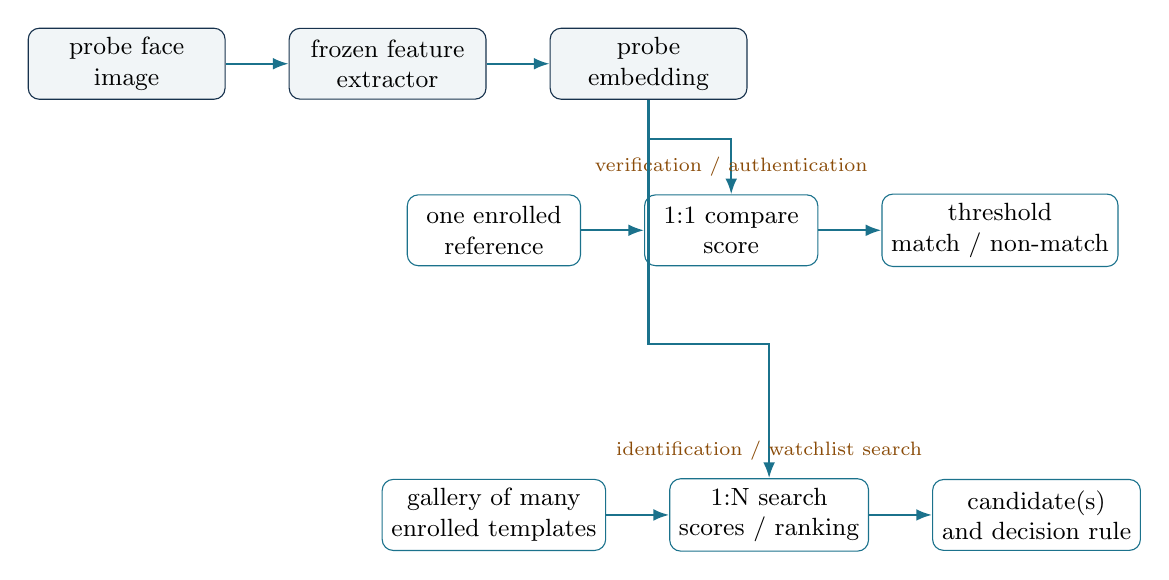
\begin{tikzpicture}[
node distance=6mm and 8mm,
box/.style={draw=navy,rounded corners,fill=soft,align=center,minimum width=25mm,minimum height=9mm,font=\small},
smallbox/.style={draw=teal,rounded corners,align=center,minimum width=22mm,minimum height=9mm,font=\small},
arr/.style={-{Latex[length=2mm]},thick,color=teal}
]
\node[box] (probe) {probe face\\image};
\node[box,right=of probe] (extract) {frozen feature\\extractor};
\node[box,right=of extract] (emb) {probe\\embedding};
\draw[arr] (probe)--(extract);\draw[arr] (extract)--(emb);

\node[smallbox,below left=12mm and -4mm of emb] (ref) {one enrolled\\reference};
\node[smallbox,right=of ref] (cmp11) {1:1 compare\\score};
\node[smallbox,right=of cmp11] (dec11) {threshold\\match / non-match};
\draw[arr] (emb.south)--++(0,-5mm)-|(cmp11.north);
\draw[arr] (ref)--(cmp11);\draw[arr] (cmp11)--(dec11);
\node[font=\scriptsize,text=warn,above=1mm of cmp11] {verification / authentication};

\node[smallbox,below=27mm of ref] (gallery) {gallery of many\\enrolled templates};
\node[smallbox,right=of gallery] (cmp1n) {1:N search\\scores / ranking};
\node[smallbox,right=of cmp1n] (dec1n) {candidate(s)\\and decision rule};
\draw[arr] (emb.south)--++(0,-31mm)-|(cmp1n.north);
\draw[arr] (gallery)--(cmp1n);\draw[arr] (cmp1n)--(dec1n);
\node[font=\scriptsize,text=warn,above=1mm of cmp1n] {identification / watchlist search};
\end{tikzpicture}
\caption{A trained face model produces embeddings; matching happens afterward. Verification
compares a probe with one claimed reference (1:1). Identification searches a probe against a
gallery (1:N). Study 0 evaluates the 1:1 representation question; 1:N system performance is
an engineering motivation, not a measured endpoint here.}
\label{fig:biometric-pipeline}
\end{figure}

\subsection{Verification, authentication, and identification}

\textbf{Verification} asks whether a probe and a specific reference belong to the same
person: one comparison, often called 1:1. \textbf{Authentication} is a use of verification
in which the person presents or implies an identity claim, for example through an account,
credential, or identity document. \textbf{Identification} asks whether the probe matches
anyone in a gallery: 1:N. A watchlist search is therefore not merely a larger 1:1 test; its
gallery size, candidate ranking, search strategy, and false-candidate behavior require
separate 1:N evaluation \cite{nistfrte1n}.

\subsection{Scores, thresholds, FMR, FNMR, ROC AUC, and EER}

The implemented matcher uses a \emph{distance}: smaller means more similar. A threshold $t$
turns the continuous distance into a binary decision,
\[
\text{match if } d\le t,\qquad \text{non-match if } d>t.
\]
A larger distance threshold accepts more comparisons. It therefore tends to \emph{increase}
the false match rate while \emph{decreasing} the false non-match rate. A smaller threshold
does the opposite. This trade-off is why a biometric result is incomplete unless the
operating point is specified.

\begin{description}
\item[FMR -- false match rate.] Among impostor/non-mated comparison attempts, the fraction
that produce a match decision at the chosen threshold. It is a comparison-level matcher
metric; it should not automatically be equated with an end-to-end transaction-level false
acceptance rate, especially when a system adds acquisition, quality, retry, liveness, or
1:N decision logic.
\item[FNMR -- false non-match rate.] Among genuine/mated comparisons, the fraction incorrectly
rejected as non-matches. It measures one form of false rejection.
\item[ROC curve.] The receiver operating characteristic traces performance as the threshold
moves, usually plotting true-match/true-positive rate against false-match/false-positive
rate. It shows the trade-off across many operating points.
\item[ROC AUC.] The area under the ROC curve summarizes global ranking/separation over the
whole threshold range. A higher AUC can coexist with worse behavior at one particular low-FMR
operating point.
\item[EER -- equal error rate.] The operating point at which FMR and FNMR are equal (or their
closest empirical crossing). It is a convenient scalar summary, but it need not correspond
to the threshold a real application would choose.
\end{description}

The distinction is operationally important. NIST reports face-verification FNMR at explicitly
specified FMR operating points, including values far below 0.01 for some datasets and use
cases \cite{nistfrte11}. Study 0's FMR 0.01 must therefore be read as a bounded research
choice, not as a recommendation for border control, a national watchlist, or any other
production deployment.

\subsection{Why operating points and decision rules must be frozen}

Suppose two methods are compared and one researcher is allowed to move the threshold after
seeing TEST outcomes. A method can then be made to look safer by accepting more false
non-matches, or more convenient by accepting more false matches. If the target FMR, margin,
seed rule, or threshold-selection procedure is changed after seeing TEST, the scientific
question itself has moved.

This paper therefore separates exploratory design choices from post-test conclusions. The
operating target, non-inferiority tolerance, random seeds, tie policy, and TEST access rule
are fixed before the claim-bearing result is interpreted. Later sections explain the exact
values and their limitations.

\subsection{A running engineering vignette}

For a concrete motivation, imagine a hypothetical product team developing a compact edge
watchlist device. An edge/biometric engineer asks whether a local gallery can be made smaller
and faster; a biometric-performance statistician -- call him Maurice -- asks whether that
engineering gain changes the probability of a false match or false non-match beyond an
acceptable tolerance. Those are different questions and both must be answered.

The memory pressure can be real without proving that compression is safe. One million
identities with five float32 templates each require 5 million templates. The raw payload
alone is 10.24 GB at 512 dimensions and 2.56 GB at 128 dimensions, before indexing, models,
OS memory, camera buffers, encryption, or engineering headroom. That fourfold arithmetic
saving gives the engineer a reason to investigate compression. Maurice's role is to prevent
the product team from turning that attractive saving into a biometric claim without a
frozen operating point, adequate data, uncertainty analysis, and independent review. Study 0
is the first controlled experiment in that chain, not a product qualification.

\section{From high-dimensional features to smaller representations}\label{sec:reduction}

The phrase \emph{feature reduction} covers several different operations. They should not be
conflated because they preserve different properties and make different assumptions.

\subsection{Feature selection versus feature extraction}

\textbf{Feature selection} keeps a subset of the original coordinates. If a vector
$z\in\mathbb{R}^{D}$ is reduced to $d$ coordinates, the output is literally a subset of
entries of $z$. This can preserve interpretability when coordinates have semantic meaning,
but modern deep embeddings usually distribute information across many coordinates, so
coordinate selection is not an obvious baseline here.

\textbf{Feature extraction} constructs new coordinates from the original ones. Linear
projections such as PCA, random projection, LDA, and the Siamese head studied here all fall
in this category. Nonlinear autoencoders are another example. The initial experiment
focuses on linear 512-to-128 extraction so that the output dimension and capacity remain
comparable across routes.

\subsection{Principal-component analysis}

PCA is an unsupervised linear method that finds orthogonal directions of maximal variance
\cite{jolliffe2016}. Let training embeddings be $z_1,\ldots,z_n$ with mean $\mu$. Define the
sample covariance
\begin{equation}
S=\frac{1}{n-1}\sum_{i=1}^{n}(z_i-\mu)(z_i-\mu)^T.
\end{equation}
If $v_1,\ldots,v_D$ are eigenvectors of $S$ ordered by decreasing eigenvalue, the
$d$-dimensional PCA representation is
\begin{equation}
u=P_d^T(z-\mu),\qquad P_d=[v_1,\ldots,v_d].
\end{equation}
PCA minimizes squared linear reconstruction error among rank-$d$ orthogonal projections and
retains directions with the most variance. It uses no genuine/impostor labels. That is both
its strength and its limitation for biometric verification: high variance is not identical
to identity-discriminative variance, and the low-FMR decision boundary is not part of the
PCA objective.

In this repository PCA is fitted only on TRAIN endpoints, with 128 components, using
scikit-learn's randomized SVD solver and a fixed seed. The projected outputs are then
L2-normalized before distances are evaluated. PCA is therefore the central unsupervised
control: if Siamese training adds value, it should do more than this ordinary data-adaptive
linear compressor at the same output dimension.

For readers who want a less formal refresher before the eigendecomposition, Andrew Ng's
Machine Learning Specialization includes a short PCA treatment in Course 3, Week 2
(``Unsupervised Learning, Recommenders, Reinforcement Learning'') \cite{ngmls}. It is cited
here as a pedagogical companion; the scientific definition and implementation in this paper
do not depend on the course.

\subsection{Random projection}

A random projection uses a matrix $R\in\mathbb{R}^{D\times d}$ that is sampled independently
of the data. In the implemented route,
\begin{equation}
R_{kl}\sim\mathcal{N}(0,1/d),\qquad u=\operatorname{normalize}(zR).
\end{equation}
Random-projection theory, including the Johnson--Lindenstrauss result, shows that a finite
set of points can often be embedded into a lower-dimensional Euclidean space while
approximately preserving pairwise distances when $d$ is sufficiently large relative to the
logarithm of the number of points \cite{johnson1984,dasgupta2003}. The theorem is not a
biometric performance guarantee, but it explains why a data-independent projection is a
useful control rather than a meaningless straw man.

The random route isolates a simple question: how much of the observed behavior comes from
reducing dimensionality alone? If a learned 128D route does not consistently beat a seeded
random 128D route under matched evaluation, the evidence for supervision-specific value is
weak.

\subsection{Other reduction families not tested in the initial experiment}

The wider design space is substantially larger than PCA and random projection:

\begin{description}
\item[Linear discriminant analysis (LDA).] LDA is supervised and seeks directions that
increase between-class separation relative to within-class variation \cite{fisher1936}.
It uses class labels rather than the pairwise contrastive objective studied here.
\item[Autoencoders.] A nonlinear encoder-decoder can learn a low-dimensional bottleneck by
minimizing reconstruction error, and deeper autoencoders can capture nonlinear structure
\cite{hinton2006}. Reconstruction quality, however, is not automatically equivalent to
low-FMR verification quality.
\item[Metric-learning projections.] Supervised objectives can learn a transformation so
that task-relevant distances are improved. Siamese contrastive learning is one member of
this family; triplet losses and large-margin metric-learning objectives are alternatives.
\item[Hashing and binary embeddings.] These reduce both representation size and the form of
the comparison operation, often replacing floating-point distances with Hamming distance.
They change more than dimensionality and therefore require a separate matched study.
\item[Quantization.] Float32 values may be converted to float16, int8, product-quantized, or
otherwise coded with fewer bits. Quantization reduces precision and storage per coordinate,
not necessarily the number of coordinates. It is complementary to dimensionality reduction
and is intentionally outside the initial experiment.
\item[End-to-end compact backbones.] A network can be trained to emit 128D directly, or the
extractor itself can be pruned, distilled or redesigned. That intervention changes the
source representation and compute graph, unlike the post-extractor projections studied
here.
\end{description}

Table~\ref{tab:methods-landscape} summarizes why the four implemented routes are useful
controls within this larger landscape.

\begin{table}[ht]
\centering
\caption{Dimensionality-reduction landscape and the role of the implemented controls.}
\label{tab:methods-landscape}
\small
\begin{tabularx}{\linewidth}{@{}p{0.18\linewidth}p{0.13\linewidth}X X@{}}
\toprule
Method & Supervision & Main optimization idea & Role in this experiment\\
\midrule
Raw 512D & none & no compression & reference performance and storage\\
Random 128D & none & data-independent distance-preserving projection & dimension-only control\\
PCA 128D & none & maximize retained variance / minimize linear reconstruction error & ordinary unsupervised compression control\\
Siamese 128D & pair labels & pull genuine pairs together, push close impostor pairs apart & test added value from pair supervision\\
LDA & identity labels & between-class versus within-class separation & not tested\\
Autoencoder & usually none & nonlinear reconstruction through a bottleneck & not tested\\
Quantization & none or learned & fewer bits per coordinate/codebook approximation & orthogonal intervention, not tested\\
\bottomrule
\end{tabularx}
\end{table}

\section{What the Siamese route actually is}\label{sec:siamese}

\subsection{Pairs first: what is being contrasted?}

The motivating public implementation is Antonio Diaz-Cano's educational
\code{siamese-network} repository, pinned here to commit
\code{6ff8abb6890dca880f8b8d2a7a90a94124b91698} \cite{diazcano2026}. The present repository
independently reproduces the experimental idea rather than copying that source code.

Siamese training starts from \emph{pairs}. A \textbf{genuine pair} contains two face samples
of the same identity, for example two photographs of person A. An \textbf{impostor pair}
contains samples from different identities, for example person A and person B. The label does
not say ``this is Alice'' or ``this is Bob''; it says only ``same identity'' or ``different
identity''. The learning problem is therefore about geometry and similarity, not closed-set
identity classification.

\subsection{Why it is called Siamese}

A Siamese architecture processes the two members of a pair through \emph{the same}
transformation. The word ``Siamese'' refers to weight sharing between twin training branches,
not to two different models. In the present experiment, each branch receives a frozen 512D
source embedding and applies the same trainable affine projection.

After that projection, the code performs \textbf{L2 normalization}. This is not a learned
neural layer in the present implementation: it has no trainable parameters. It simply rescales
a vector to length one while preserving its direction. If $x=(3,4)$, for example,
$\|x\|_2=5$ and its L2-normalized version is $(0.6,0.8)$. Formally,
\begin{equation}
\tilde u = zW+b,\qquad u=\frac{\tilde u}{\|\tilde u\|_2},
\end{equation}
where $W\in\mathbb{R}^{512\times128}$ and $b\in\mathbb{R}^{128}$. The two branches share the
same $W$ and $b$. The head therefore has
\begin{equation}
512\times128+128=65{,}664
\end{equation}
trainable parameters.

\begin{figure}[ht]
\centering
\resizebox{\linewidth}{!}{%
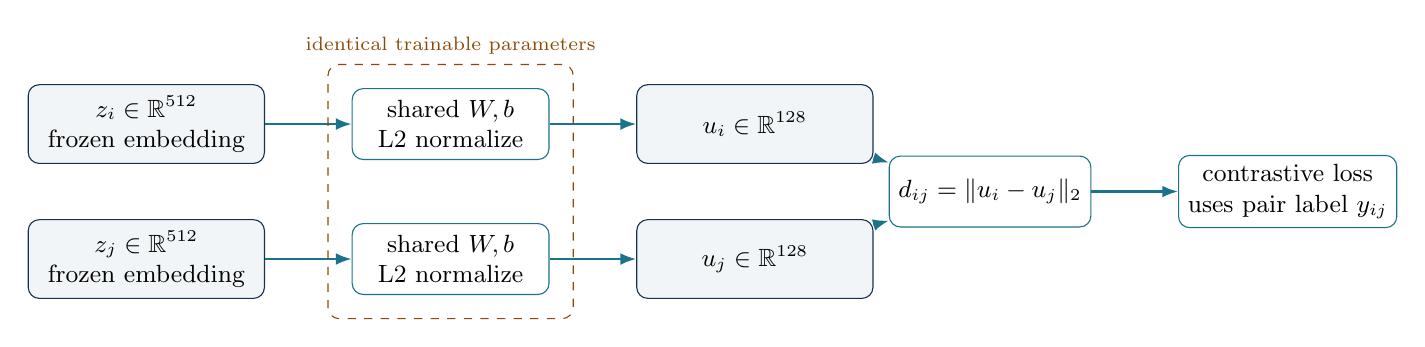
\begin{tikzpicture}[
node distance=7mm and 11mm,
box/.style={draw=navy,rounded corners,fill=soft,align=center,minimum width=30mm,minimum height=10mm,font=\small},
smallbox/.style={draw=teal,rounded corners,align=center,minimum width=25mm,minimum height=9mm,font=\small},
arr/.style={-{Latex[length=2mm]},thick,color=teal}
]
\node[box] (z1) {$z_i\in\mathbb{R}^{512}$\\frozen embedding};
\node[box,below=of z1] (z2) {$z_j\in\mathbb{R}^{512}$\\frozen embedding};
\node[smallbox,right=of z1] (g1) {shared $W,b$\\L2 normalize};
\node[smallbox,right=of z2] (g2) {shared $W,b$\\L2 normalize};
\node[box,right=of g1] (u1) {$u_i\in\mathbb{R}^{128}$};
\node[box,right=of g2] (u2) {$u_j\in\mathbb{R}^{128}$};
\node[smallbox,right=17mm of $(u1)!0.5!(u2)$] (dist) {$d_{ij}=\|u_i-u_j\|_2$};
\node[smallbox,right=of dist] (loss) {contrastive loss\\uses pair label $y_{ij}$};
\draw[arr] (z1)--(g1);\draw[arr] (z2)--(g2);
\draw[arr] (g1)--(u1);\draw[arr] (g2)--(u2);
\draw[arr] (u1)--(dist);\draw[arr] (u2)--(dist);\draw[arr] (dist)--(loss);
\node[draw=warn,dashed,rounded corners,fit=(g1)(g2),inner sep=3mm,label={[font=\scriptsize,text=warn]above:identical trainable parameters}] {};
\end{tikzpicture}%
}
\caption{Training view of the implemented Siamese projection. The two pair members use the
same trainable projection. The pair label influences the loss, and the loss updates those
shared parameters.}
\label{fig:siamese}
\end{figure}

\subsection{Euclidean distance versus cosine similarity after L2 normalization}

L2 normalization puts every output vector on the unit sphere. For unit vectors $u_i$ and
$u_j$, their dot product is their cosine similarity, and Euclidean distance is linked to it
exactly:
\begin{equation}
\|u_i-u_j\|_2^2 = 2-2\,u_i^T u_j = 2\bigl(1-\cos(u_i,u_j)\bigr).
\end{equation}
This means the two measures contain the same ordering information after normalization, but
their numeric scales and directions differ. A large cosine similarity means a small
Euclidean distance. For example, cosine similarity $0.8$ corresponds to Euclidean distance
$\sqrt{2-2(0.8)}\approx0.632$. A cosine rule ``match if similarity is at least 0.8'' therefore
corresponds exactly to the Euclidean rule ``match if distance is at most 0.632'' for unit
vectors.

The implementation in this repository computes and thresholds \emph{Euclidean distance}.
Calling the matcher ``cosine-based'' would be acceptable only as shorthand for this
one-to-one monotonic relation on normalized vectors; it would be misleading if it suggested
that the code actually thresholds a cosine value. The paper therefore reports the implemented
Euclidean distance explicitly.

\subsection{Contrastive training objective}

Here \emph{contrastive} means that learning is driven by contrasting two kinds of pairs:
genuine pairs should become close, while impostor pairs that are too close should be pushed
apart. The broader Siamese idea goes back at least to shared-weight signature verification
\cite{bromley1993}; discriminative similarity learning was later applied directly to face
verification \cite{chopra2005}, and the margin-based contrastive formulation used here is
closely associated with invariant mapping work by Hadsell, Chopra, and LeCun
\cite{hadsell2006}.

For pair label $y_{ij}=1$ when the two samples share an identity and $y_{ij}=0$ otherwise,
the implemented loss is
\begin{equation}
\mathcal{L}_{ij}=\frac{1}{2}y_{ij}d_{ij}^{2}
+\frac{1}{2}(1-y_{ij})\max(0,m-d_{ij})^{2},
\end{equation}
with margin $m=1$. Genuine pairs are penalized in proportion to squared distance, so the
optimizer pulls them together. Impostor pairs are penalized only when they lie inside the
margin; once they are at least $m$ apart, this loss applies no further pressure to separate
them.

Training uses mini-batches of pairs, Adam-style moment updates, weight decay, and early
stopping on validation contrastive loss. The LFW configuration allows up to 60 epochs, batch
size 128, learning rate $10^{-3}$, weight decay $10^{-4}$, patience 8 and minimum validation
improvement $10^{-4}$. These choices are frozen before TEST evaluation.

\subsection{Training versus inference -- the shortest operational distinction}

The easiest way to separate the two phases is to ask whether model parameters are still
being changed. During \textbf{training}, labelled pairs create a loss and the optimizer
updates $W,b$. During \textbf{inference}, the parameters are fixed: a face produces one
embedding, and matching compares fixed embeddings. There is no pair label, no loss, and no
optimizer.

\begin{table}[ht]
\centering
\caption{Training and inference are different operations even though they use the same
learned projection.}
\label{tab:train-infer}
\small
\begin{tabularx}{\linewidth}{@{}p{0.20\linewidth}XX@{}}
\toprule
 & Training & Inference / deployment\\
\midrule
Input & labelled genuine/impostor pairs & one probe face at a time, plus stored reference/gallery templates\\
Shared projection & used in two branches & used once per face/template\\
Pair label & required & absent\\
Contrastive loss & computed & absent\\
Optimizer / weight update & yes & no\\
Output of the phase & learned parameters $W,b$ & fixed 128D template and later a match/search score\\
Decision threshold & not the learning target itself & applied to scores according to the operating policy\\
\bottomrule
\end{tabularx}
\end{table}

After training, a single source embedding follows
\begin{equation}
z\longmapsto u=\operatorname{normalize}(zW+b).
\end{equation}
The resulting 128D template can be stored. Verification later compares a probe with one
reference; identification could search a gallery. The two-branch training construction does
not mean that deployment requires a special two-network runtime.

The experiment is also not closed-set identity classification. No softmax head predicts one
of the training identities. Pair supervision says only whether two training samples share an
identity. This is why Siamese learning naturally supports verification and open-set matching
\cite{bromley1993,koch2015}.

\subsection{What the Siamese route is meant to prove -- and what it cannot prove by itself}

The Siamese route tests whether pairwise supervision can learn a better 128D linear geometry
than unsupervised or data-independent reduction. It does \emph{not} prove useful compression
merely because contrastive loss decreases. It must still satisfy the downstream verification
endpoint and must be compared with raw, random and PCA controls at the same output dimension.

This is why the baseline hierarchy matters:
\begin{itemize}
\item raw versus Siamese asks whether the learned compression preserves enough performance;
\item random versus Siamese asks whether supervision adds more than dimension reduction alone;
\item PCA versus Siamese asks whether supervision adds more than an ordinary data-adaptive linear compressor;
\item secondary AUC or EER improvements cannot override a failed predeclared low-FMR endpoint.
\end{itemize}

\section{Experimental object and matched routes}\label{sec:object}

A frozen ImageNet-pretrained ResNet-18 maps each LFW image to a 512D feature vector. The
original classification layer is replaced with an identity map, so the penultimate 512D
representation is retained. Images are resized to $224\times224$ and normalized with the
standard ImageNet channel statistics. The extractor is frozen; no face-specific fine-tuning
occurs.

Each route receives the same frozen source embeddings and the same pair splits. Raw and
random routes have no fitted parameters. PCA is fitted only on TRAIN endpoints. The Siamese
head is fitted on TRAIN pairs with early stopping on VALIDATION. All outputs are L2-normalized
before Euclidean distance is measured.

This design isolates the post-extractor compression intervention. It deliberately does not
ask whether a different face backbone, end-to-end compact network, nonlinear head or
quantized representation would perform better.

\subsection{Why the ImageNet ResNet-18 starting point is pedagogical, not a face-recognition baseline}\label{sec:backbone-provenance}

The starting architecture was inherited deliberately from the public educational
implementation that motivated this work \cite{diazcano2026}. In that implementation, a
torchvision ResNet-18 initialized with ImageNet classification weights is used as the shared
backbone; every ResNet parameter is frozen, and only the final 512-to-128 embedding head is
trainable. The present repository independently reproduces that experimental idea. Thus it
would be inaccurate to say that a ResNet-18 face recognizer was ``trained on LFW''. The
ResNet-18 had already been trained for ImageNet object classification; LFW pair supervision
trained only the small projection placed on top of its 512D penultimate features.

This is a useful pedagogical construction because it isolates metric learning: the source
representation is fixed, so any difference among raw, random, PCA and Siamese routes is due
to the post-extractor transformation. It is not, however, a strong way to establish face
verification performance. ImageNet supervision rewards separation of generic object
categories, not identity discrimination among faces under changes of age, pose,
illumination, expression, occlusion and capture quality. A frozen linear head can reweight
and rotate information already present in the 512D vector, but it cannot recover identity
information that the ImageNet extractor never encoded reliably. The preprocessing is
likewise generic ImageNet resize/normalization applied to LFW-deepfunneled imagery; the
experiment does not evaluate a modern face-detection/alignment/quality pipeline as part of
the source representation.

The remembered ``about 70 percent accuracy'' is directionally consistent with the immutable
replay, but accuracy optimized on TEST is not the scientific endpoint. If a decision
threshold is chosen directly on TEST to maximize pair classification accuracy, the Study 0
scores give 71.5\% for raw 512D, 73.0--74.7\% across the five Siamese seeds, and
74.1--74.3\% for PCA. These are descriptive, TEST-tuned values and therefore optimistic for
deployment. Their value here is diagnostic: absolute face-verification performance is weak
enough that the source backbone should be questioned before a compression failure is
attributed to the 128D projection itself.

Modern face-recognition systems instead learn identity-discriminative embeddings with
face-specific objectives and data. Representative families include FaceNet-style metric
learning \cite{facenet2015} and angular-margin classification such as ArcFace
\cite{arcface2019}; quality-aware variants such as AdaFace \cite{adaface2022} adapt the
learning objective to image quality. The next experiment therefore changes the source
representation before asking the compression question again.

\section{The initial experiment}\label{sec:initial}

\subsection{Data and splits}

The benchmark follows the LFW development protocol \cite{lfw2007}. The executed split
contains 842 training pairs, 795 validation pairs, and 1,000 untouched DevTest pairs.
DevTest contains 500 genuine and 500 impostor pairs and 963 distinct endpoint identities.
Development and test identities are kept separate according to the frozen protocol.

This setup is deliberately limited. With 500 impostor pairs, empirical FMR changes in steps
of $1/500=0.002$. It cannot establish claims at $10^{-4}$, $10^{-5}$, or national-scale
operating points. ImageNet ResNet-18 is also not a biometric-grade face extractor. The
experiment is therefore a controlled representation study, not a production benchmark.

\subsection{Why there are two threshold questions}

A matcher does not directly output ``same person'' or ``different person''; it outputs a
score. In this implementation, smaller Euclidean distance means greater similarity. Choosing
a threshold is therefore part of the question being asked. If the threshold is loosened,
more genuine pairs pass but more impostor pairs can also pass. If it is tightened, false
matches tend to fall while false non-matches tend to rise.

That creates two scientifically different questions:

\textbf{1. Equal-FMR representation benchmark.} If raw 512D and a compressed route are each
allowed their own TEST threshold so that both operate at the same empirical FMR target, which
representation has the lower FNMR? This isolates discrimination at a common error budget.
The threshold is intentionally located on TEST, so this analysis is a \emph{representation
benchmark}, not a deployable threshold-setting procedure.

\textbf{2. Validation-frozen threshold transfer.} If a threshold is selected using
VALIDATION only, frozen, and then applied unchanged to TEST, what FMR and FNMR result? This
asks whether calibration transfers to new data. Because each route can land at a different
TEST FMR, these rows must not be ranked as if they were equal-FMR comparisons.

Both questions are useful. The first compares representations at a matched operating point;
the second is closer to how a real threshold would have to be chosen before production data
are observed.

\subsection{From an engineering tolerance to a non-inferiority rule}

The primary Study 0 question is not ``is 128D better than 512D?'' It is ``is the loss, if
any, small enough to be tolerated?'' We call that a \textbf{non-inferiority} question in the
rest of the paper. A non-inferiority design declares a maximum acceptable degradation
$\delta$ before looking at the claim-bearing result and asks whether the data support keeping
the degradation below that margin \cite{wellek2010}.

Study 0 first fixes the false-match operating point at
\[
\alpha=0.01.
\]
Here $\alpha$ is simply notation for the target FMR; it is \emph{not} a hypothesis-test
significance level. FMR 0.01 means 1\% of impostor comparisons. On 500 DevTest impostor
pairs, the empirical grid moves in increments of 0.002, so 0.01 corresponds nominally to
five false matches out of 500. The frozen tie policy keeps equal-distance blocks together,
so the selected empirical FMR can be below 0.01 if a tied block cannot be included without
exceeding the target.

Why 0.01? It is low enough to focus the experiment away from a purely global AUC/EER summary
while still being resolvable on only 500 impostor pairs. It is \emph{not} claimed to be an
appropriate production threshold. Current large-scale face evaluations commonly report
performance at much lower FMR values for security-sensitive use cases \cite{nistfrte11}.
Study 0 simply cannot resolve those regimes with its sample size.

At that same empirical FMR, define for candidate route $m$ and raw reference $b$
\begin{equation}
\DeltaFNMR(m,\alpha)=\fnmr_m(\alpha)-\fnmr_b(\alpha).
\end{equation}
A positive value means the compressed route rejects more genuine comparisons than raw. The
frozen non-inferiority margin is
\[
\delta=0.03,
\]
meaning an additional \textbf{three absolute percentage points of FNMR}. The repository does
not contain a product- or regulation-derived argument that 3 percentage points is universally
acceptable; it is a preregistered exploratory tolerance for this study. A future operational
study must justify its margin from the real use case, costs of errors, population, sensors,
and decision policy rather than inheriting 0.03 by habit.

The corrected bootstrap produces a two-sided 95\% percentile interval for $\DeltaFNMR$; the
97.5th percentile is its upper endpoint. A candidate seed passes only if even that upper
bound is no larger than the allowed degradation:
\begin{equation}
\operatorname{UCB}_{0.975}\left[\DeltaFNMR(m,0.01)\right]\le 0.03.
\end{equation}
In plain language: the point estimate is not enough. The uncertainty must also fit below the
engineering tolerance.

\subsection{What ``predeclared seed'' means}

Machine-learning experiments often contain pseudo-random operations: initialization of a
learned projection, generation of a random-projection matrix, randomized numerical solvers,
or the ordering/sampling used during training. A \textbf{random seed} is the integer that
initializes the pseudo-random number generator. Fixing it makes a stochastic run replayable;
changing it gives another legitimate realization of the same algorithm.

The stochastic 128D routes use seeds $\{11,29,47,71,101\}$. \textbf{Predeclared} means these
values and the rule for using them were fixed before TEST outcomes were inspected. Study 0
requires \emph{every} declared seed to pass. This deliberately prevents ``seed shopping'':
running many variants and reporting only the random realization that happened to look best
on TEST. Reproducibility guidance in machine learning similarly treats random-state reporting
as part of the experiment rather than an incidental implementation detail \cite{pineau2021}.

\section{Why the original uncertainty analysis was not sufficient}\label{sec:defect}

\subsection{The intuition: pair rows can share the same person}

A bootstrap approximates sampling variability by repeatedly constructing resampled versions
of the observed data and recomputing the statistic \cite{efron1993}. The crucial question is
\emph{what unit should be resampled?} If observations are independent people, resampling
people is natural. If several table rows are linked through the same person, resampling rows
as if they were independent can misrepresent uncertainty.

In face verification, one identity can appear in several pair comparisons. Figure
\ref{fig:pair-dependence} gives a toy example. Two images of identity A form a genuine pair;
images of A also participate in impostor pairs with identities B and C. If identity A is
unusually easy or hard for the matcher, several pair scores can move together. Three pair
rows therefore do not automatically represent three independent person-level observations.

\begin{figure}[ht]
\centering
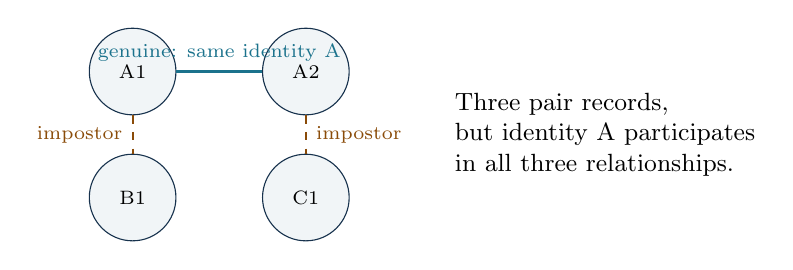
\begin{tikzpicture}[
img/.style={draw=navy,circle,fill=soft,minimum size=11mm,align=center,font=\scriptsize},
arrg/.style={thick,color=teal},
arri/.style={thick,dashed,color=warn}
]
\node[img] (a1) at (0,0) {A1};
\node[img] (a2) at (2.2,0) {A2};
\node[img] (b1) at (0,-1.6) {B1};
\node[img] (c1) at (2.2,-1.6) {C1};
\draw[arrg] (a1)--node[above,font=\scriptsize]{genuine: same identity A}(a2);
\draw[arri] (a1)--node[left,font=\scriptsize]{impostor}(b1);
\draw[arri] (a2)--node[right,font=\scriptsize]{impostor}(c1);
\node[align=left,font=\small] at (6.0,-0.8) {Three pair records,\\but identity A participates\\in all three relationships.};
\end{tikzpicture}
\caption{Toy dependence structure. Resampling pair rows independently can ignore repeated
identity involvement. The corrected Study 0 procedure resamples subject slots and then
reweights only the pair edges that were actually observed.}
\label{fig:pair-dependence}
\end{figure}

\subsection{What the historical analysis did}

The historical execution resampled genuine-pair indices and impostor-pair indices with
replacement. Candidate and raw routes used the same sampled indices, so the comparison was
paired across matchers and stratified by label. However, the estimator treated pair records
as the resampling unit even when multiple records shared an identity. The research contract
had described the uncertainty as identity-aware. The executed estimator therefore did not
match the declared sampling unit. This discrepancy was recorded as E-STAT-001. The original
scores, tables, paper, and negative decision were retained rather than overwritten.

This distinction matters even if a corrected analysis later reaches the same qualitative
conclusion. In the present one-sided non-inferiority decision, an interval that is too narrow
creates a particular risk of \emph{false confidence}: near the 0.03 boundary it could make
an upper confidence bound appear to fit below the margin when a correctly calibrated
subject-level interval would not. More generally, a wrong dependence model can distort
coverage in either direction. In this dataset the corrected intervals became wider and the
high-level decision remained negative, so no positive claim was rescued or created by the
correction.

The correction question was therefore not ``can the old answer be reproduced?'' but ``does
a subject-level estimator with demonstrated coverage change the decision?''

\section{Frozen correction}\label{sec:correction}

\subsection{Subject bootstrap before the implementation details}

A \textbf{subject bootstrap} resamples identities rather than pretending every pair row is an
independent experimental unit. ``With replacement'' means that, in one bootstrap replicate,
an identity can be drawn zero times, once, or several times. Repeating this many times creates
a distribution of the statistic that reflects which people happened to be represented in
the sample. No new face images are synthesized and no model is retrained.

Study 0 needs one extra device because its TEST data are a sparse graph of observed pairs,
not a complete all-pairs matrix. The frozen solution is a \textbf{weighted subject-slot
bootstrap}: draw subject slots with replacement, then use the draw multiplicities to weight
only the genuine and impostor edges that actually existed in DevTest. This preserves the
historical comparison graph rather than inventing unobserved impostor pairs.

\subsection{Weighted subject-slot bootstrap}

The correction operates on the exact historical score table and the observed LFW DevTest
pair graph. No model is retrained and no historical score is recomputed.

For each replicate, 963 subject slots are drawn with replacement. Let $m_i$ be the
multiplicity of subject $i$ in that draw. The frozen weighting rule is:
\begin{align}
  w_{ij}^{\mathrm{genuine}} &= m_i,\\
  w_{ij}^{\mathrm{impostor}} &= m_i m_j.
\end{align}
For a genuine edge, repeated sampling of its identity contributes proportionally to that
identity's multiplicity. For an observed impostor edge between subjects $i$ and $j$, the
weight is the product of their multiplicities because each resampled copy of $i$ can pair
with each resampled copy of $j$ along that already-observed edge.

Only observed DevTest edges are weighted; no missing all-pairs comparison is synthesized.
Candidate and raw routes use the same subject draw, preserving pairing between methods. The
implementation uses PCG64 and 10,000 bootstrap replicates per seed, with convergence
checkpoints at 2,000, 5,000 and 10,000 replicates. Degenerate replicates fail the reanalysis
rather than being silently redrawn.

The representation endpoint recalibrates each route within each replicate to the frozen
equal-FMR benchmark rule. A separate operational bootstrap keeps the VALIDATION-selected
threshold fixed while estimating TEST FNMR and FMR uncertainty.

\subsection{Known-truth coverage validation}

A 95\% interval procedure is useful only if it actually covers the true value with roughly
the advertised frequency under relevant repeated-sampling regimes. Real biometric data do
not reveal the true population parameter, so the corrected procedure was first tested on
synthetic sparse pair graphs where the truth is known by construction.

The simulations preserve the 963-subject, 500-genuine, 500-impostor structure. Five
predeclared regimes included independent-pair and subject-dependent nulls, non-inferior,
boundary, and inferior cases. Coverage was assessed separately for the representation
delta-FNMR and for operational FNMR and FMR.

The simulation stopped at 4,000 independently generated datasets per scenario once the
Monte Carlo standard-error rule was satisfied. All 15 scenario-by-metric coverage checks met
the frozen criterion. The weakest exact 95\% Clopper--Pearson lower bound was 0.937743,
above the required 0.93. This validation supports the interval procedure under the specified
synthetic regimes; it does not by itself establish anything about the value of
128-dimensional compression.

\section{Replay, provenance, and independent verification}\label{sec:verification}

The corrected analysis was bound to the immutable historical run
\begin{quote}
\code{lfw\_resnet18\_siamese\_projection\_v0\_1-89179914-911192ee-64559cbd}.
\end{quote}
The recovered historical replay archive is 4,158,610 bytes with SHA-256
\texttt{\seqsplit{7429c75a7da827281ca172d7a4184c65fcc27dbfa845eb9ffd27e04d81331897}}.
Its preserved \code{test\_pair\_scores.csv} is 1,821,547 bytes and has SHA-256
\texttt{\seqsplit{f52ea23987a9d22647e0f63275a3d8a215b5fb0c588bac41723298537b383439}}.

The corrected materialization records the runner commit, frozen configuration, source
hashes, output hashes, and the fact that the historical inputs were not mutated. An
independent reviewer recalculated all declared artifact hashes, verified the original
archive identity and the copied known-truth coverage evidence, and confirmed that the
successful materialization came from a fresh run rather than from a previously interrupted
partial directory.

Only after those provenance checks were complete were numerical result tables opened for
interpretation. A second independent review recalculated the numerical claims reported in
this paper directly from the materialized result files, checked the decision rule, verified
that validation thresholds remained validation-derived, and examined convergence from
2,000 to 10,000 bootstrap replicates. No discrepancies requiring a change to the
interpretation were found.

This verification chain is intentionally described in prose rather than as a process badge:
the scientific value comes from what was independently recalculated and checked, not from a
status label.

\section{Corrected results}\label{sec:results}

\subsection{Primary non-inferiority endpoint}

Table~\ref{tab:ni} gives the corrected all-seeds result. No 128D route satisfies the frozen
non-inferiority criterion on any of its five predeclared seeds.

\begin{table}[ht]
\centering
\caption{Corrected subject-bootstrap non-inferiority result at empirical FMR 0.01. A seed
passes only if its 97.5\% upper bound for $\DeltaFNMR$ is at most 0.03.}
\label{tab:ni}
\begin{tabular}{@{}lcc@{}}
\toprule
Route & Seeds passing & Range of 97.5\% UCBs\\
\midrule
Random 128D & 0/5 & 0.112649--0.151768\\
PCA 128D & 0/5 & 0.125556--0.133606\\
Siamese 128D & 0/5 & 0.176584--0.189156\\
\bottomrule
\end{tabular}
\end{table}

For the Siamese route, the observed equal-FMR point deltas across the five seeds are
\[
+0.034,\quad +0.064,\quad -0.006,\quad +0.050,\quad +0.010,
\]
and the corresponding subject-bootstrap means are
\[
+0.0392,\quad +0.0438,\quad +0.0024,\quad +0.0372,\quad +0.0113.
\]
One point estimate is slightly favorable to the candidate, but the decision rule is based on
uncertainty and all predeclared seeds. Every upper bound is well above 0.03. The admissible
conclusion is therefore \emph{failure to demonstrate non-inferiority}, not proof of
inferiority.

\subsection{What changed after correcting the sampling unit}

Table~\ref{tab:widths} compares average 95\% interval widths from the historical pair
bootstrap and the corrected subject bootstrap.

\begin{table}[ht]
\centering
\caption{Average 95\% interval width for $\DeltaFNMR$.}
\label{tab:widths}
\begin{tabular}{@{}lccc@{}}
\toprule
Route & Pair bootstrap & Subject bootstrap & Width ratio\\
\midrule
Random 128D & 0.1304 & 0.2042 & $\approx1.57\times$\\
PCA 128D & 0.1749 & 0.2664 & $\approx1.52\times$\\
Siamese 128D & 0.1944 & 0.2991 & $\approx1.54\times$\\
\bottomrule
\end{tabular}
\end{table}

The original pair-level analysis materially understated uncertainty for this sample. The
correction does not reverse the negative decision, but it changes how confident one should
be about seed-level differences. This is a substantive statistical result even though the
high-level claim status is unchanged.

\subsection{Validation-frozen threshold transfer}

At thresholds selected on VALIDATION and then transferred unchanged to TEST, the bootstrap
means averaged across available seeds are approximately:

\begin{table}[ht]
\centering
\caption{Validation-frozen operational threshold transfer. Different TEST FMR values mean
these rows are not an equal-FMR ranking.}
\label{tab:operational}
\begin{tabular}{@{}lcc@{}}
\toprule
Route & FNMR & FMR\\
\midrule
Raw 512D & 0.8939 & 0.00201\\
PCA 128D & 0.8468 & 0.00201\\
Random 128D & 0.8940 & 0.00241\\
Siamese 128D & 0.9311 & 0.00158\\
\bottomrule
\end{tabular}
\end{table}

For the Siamese route, the transferred threshold produces a lower observed FMR together
with a higher FNMR than raw. That is a stricter operating trade-off, not evidence that the
primary equal-FMR non-inferiority claim was recovered.

\subsection{Secondary descriptive metrics from the historical execution}

For completeness, the original equal-FMR TEST summaries are shown in
Table~\ref{tab:secondary}. These are descriptive and do not override the primary corrected
non-inferiority decision.

\begin{table}[ht]
\centering
\caption{Historical descriptive TEST equal-FMR metrics at FMR 0.01.}
\label{tab:secondary}
\begin{tabular}{@{}lccc@{}}
\toprule
Route & FNMR mean & ROC AUC mean & EER mean\\
\midrule
Raw 512D & 0.8060 & 0.7931 & 0.2890\\
PCA 128D & 0.8216 & 0.8058 & 0.2704\\
Random 128D & 0.8416 & 0.7726 & 0.3104\\
Siamese 128D & 0.8288 & 0.8167 & 0.2662\\
\bottomrule
\end{tabular}
\end{table}

The Siamese route has the highest mean AUC and lowest mean EER in this historical table, but
that pattern is not sufficient to establish preservation at the low-FMR endpoint. Nor does
this experiment contain a preregistered superiority margin or Pareto rule by which Siamese
could be declared superior to PCA or random projection.

\section{Scientific interpretation}\label{sec:interpretation}

The corrected experiment supports four bounded conclusions.

\begin{enumerate}
\item The implemented pair-supervised objective genuinely updates a shared linear
      projection; the mechanism is real.
\item The tested 128D routes do not demonstrate non-inferiority to raw 512D under the frozen
      all-seeds rule at empirical FMR 0.01.
\item Pair supervision does not demonstrate added compression value over matched PCA and
      random controls in this experiment.
\item The original pair bootstrap understated uncertainty relative to the corrected
      subject-level analysis, while the qualitative negative decision remained unchanged.
\end{enumerate}

The statistical defect is therefore resolved for the corrected reanalysis: the estimator
matches the declared subject-level sampling unit, its coverage was validated under frozen
known-truth scenarios, the exact historical scores were reanalysed without recomputation,
and the result was independently recalculated. This validates the corrected inference
procedure for the bounded experiment; it does not turn a negative claim into a positive one.

The following statements are not supported:
\begin{itemize}
\item ``128D embeddings are intrinsically worse than 512D embeddings.''
\item ``Siamese metric learning does not work.''
\item ``PCA is superior to Siamese compression in general.''
\item ``The compression is biometric-grade or suitable for industrial low-FMR use.''
\item ``A fourfold reduction in vector dimension produces a fourfold end-to-end speed-up.''
\end{itemize}

\section{Engineering value and what was actually measured}\label{sec:engineering}

For float32 templates, a 512D vector occupies 2,048 bytes and a 128D vector 512 bytes. The
payload-only template size is therefore reduced by a factor of four. The learned projection
contains $512\times128+128=65{,}664$ float32 parameters, or 262,656 bytes.

If the common extractor is excluded because it is identical for both routes, route-specific
storage is
\begin{align}
C_{\mathrm{raw}}(N) &= 2048N,\\
C_{\mathrm{proj}}(N) &= 512N + 262656.
\end{align}
The two are equal at $N=171$ templates, and the projected route is smaller above that count
under these narrow assumptions.

For the edge-watchlist vignette introduced earlier, larger galleries make the arithmetic
more tangible. Table~\ref{tab:gallery-payload} gives payload only; it deliberately excludes
index structures, identity metadata, models, runtime buffers, operating system memory,
security overhead and engineering headroom.

\begin{table}[ht]
\centering
\caption{Exact float32 template payload under several illustrative gallery sizes. These are
engineering calculations, not measurements from Study 0.}
\label{tab:gallery-payload}
\begin{tabular}{@{}lrr@{}}
\toprule
Gallery & 512D FP32 & 128D FP32\\
\midrule
100k identities $\times$ 1 template & 204.8 MB & 51.2 MB\\
500k identities $\times$ 3 templates & 3.072 GB & 0.768 GB\\
1M identities $\times$ 5 templates & 10.24 GB & 2.56 GB\\
\bottomrule
\end{tabular}
\end{table}

If the largest illustrative gallery were scanned exhaustively for every probe, those same
10.24 GB or 2.56 GB of vector payload would have to be read per query. At 1,000 probes per
hour (about 0.278 queries/s on average), payload traffic alone would be about 2.84 GB/s for
512D and 0.71 GB/s for 128D before any indexing or implementation overhead. This calculation
is intentionally naive: a real 1:N system may use approximate-nearest-neighbor indexing,
quantization, batching, accelerators, caches, or multi-stage search. Those mechanisms can
change both resource cost and recognition behavior and therefore require separate
measurement.

A separate first-pass AI-assisted mechanical exploration was run only to test whether the
engineering motivation was physically plausible enough to be worth keeping. The generated
concept allocated an enclosure of roughly $120\times68\times138$ mm, about 1.13 litres. That
is already much larger than a later aspirational ultra-thin envelope of
$100\times150\times30$ mm (0.45 litres), illustrating that camera depth, battery volume,
thermal paths, antennas and board stacking can dominate the product architecture long before
template payload is the only constraint. This generated layout is not a validated PCB,
thermal model, battery design, or biometric benchmark, and no result in Study 0 depends on it.
A dedicated edge-device study is intentionally deferred.

Study 0 measures neither feature-extraction time, projection latency, index behavior,
memory hierarchy effects, energy, nor 1:N throughput. A work proxy for exact distance search
decreases from $512N$ to $128N$ vector components, but no fourfold end-to-end speed-up follows
from dimension alone. The hardware/device concept is therefore an engineering motivation for
the research programme, not evidence contained in this experiment.

\section{Methodological lesson: screen before full qualification}\label{sec:lesson}

The long corrective chain was justified because E-STAT-001 affected evidence already being
used as a foundation for the next study. Once a foundational uncertainty contract is found
to be wrong, the correct response is to repair and replay the evidence chain rather than
quietly move on.

The same episode also exposes a cost-design lesson. Many research directions do not need
publication-grade qualification before one knows whether they contain a useful signal. A
more efficient programme separates two evidence modes:

\begin{description}
\item[Exploratory screening.] Use a dedicated screening set, matched controls, fewer
predeclared screening seeds and a bounded compute budget to answer only whether further
investment is justified. Screening evidence is explicitly not claim-bearing and never
opens the qualification TEST set.
\item[Qualification.] Only a promoted direction incurs the full burden of frozen estimands,
all qualification seeds, validated uncertainty, untouched TEST, immutable provenance,
replay, gates and independent review.
\end{description}

The principle is not ``use less rigor''. It is:
\begin{quote}
Use the minimum sufficient rigor for the decision currently being made, and escalate the
evidence burden explicitly when a result is promoted toward a scientific claim.
\end{quote}

A negative screening result is valuable if it prevents an unjustified qualification
campaign. A negative qualified result is valuable if it closes a claim under a defensible
procedure.

\section{Implications for the next experiment}\label{sec:next}

The next planned experiment replaces the ImageNet source representation with a recognized
face-specific embedding. It remains unexecuted. Its design is being amended to use the
progressive evidence model described above.

The screening stage will use a dedicated SCREEN dataset that is separate from the untouched
qualification TEST set. Raw, random, PCA and Siamese routes remain matched. Screening seeds
are fixed as $\{11,29\}$ only to control exploratory cost; they cannot be used later to drop
unfavorable qualification seeds. Before screening outcomes are opened, a numerical
promotion/stop rule must be frozen. The first question is whether the raw face-specific
backbone itself is credible at the target low-FMR operating region. The second is whether at
least one 128D route shows enough retention signal relative to raw and matched controls to
justify qualification.

\subsection{Backbone and dataset roles for the next experiment}

The preferred design is a \emph{pretrained, frozen face-specific extractor} rather than
making backbone training part of the primary compression experiment. The exact model must be
frozen before screening with architecture, preprocessing, detector/alignment pipeline,
weight digest, training corpus, licence and training provenance recorded. An ArcFace-family
iResNet is a natural candidate because its objective is explicitly identity-discriminative
\cite{arcface2019}; AdaFace is a reasonable secondary candidate if quality-aware source
features become a separately preregistered question \cite{adaface2022}. Trying many
backbones and retaining whichever looks best after SCREEN would simply move seed/model
selection bias one level upward, so any multi-backbone comparison must itself be frozen in
advance.

The data roles must also remain distinct:
\begin{itemize}
\item \textbf{Backbone-training provenance:} the corpus used to train the frozen face
      extractor is not Study 1 projection data, but it must be documented sufficiently to
      audit identity overlap with later benchmarks.
\item \textbf{Projection development (TRAIN/VALIDATION):} use a sufficiently large,
      authorized face-development corpus with many identities and captures, identity-disjoint
      from qualification. VGGFace2 is scientifically attractive for pose and age variation
      \cite{vggface2_2018}; however, the official Oxford site now states that its download
      links are no longer available \cite{vggface2site}. Study 1 must therefore not assume
      VGGFace2 is a reproducible dependency unless lawful access is actually established.
\item \textbf{Exploratory SCREEN:} benchmarks such as LFW, CFP-FP, AgeDB-30, CALFW and CPLFW
      can provide fast sanity/stress checks for frontal/profile, age and pose behavior. They
      remain non-claim-bearing. Published work documents identity overlap between common
      web-scale face-training corpora and LFW-family benchmarks \cite{overlap2024}, so
      overlap must be audited rather than assumed absent.
\item \textbf{Claim-bearing research TEST:} IJB-C 1:1 template verification is an
      established benchmark with substantially richer unconstrained imagery than LFW
      \cite{ijbc2018}, but it is no longer a generally downloadable ``public candidate''.
      NIST discontinued distribution of IJB-A/B/C on 14 March 2023 \cite{nistijb}. It can be
      considered only if lawful access already exists and the overlap/protocol contract can
      be frozen. Otherwise another preregistered corpus must meet the identity/capture count,
      low-FMR precision, provenance and disjointness requirements rather than weakening the
      gate.
\item \textbf{Operational/external validity:} no celebrity or web-photo benchmark by itself
      establishes representativity for a passport, border, mobile, event-watchlist or
      national-gallery deployment. A later study requires authorized data that match the
      intended population, sensor, capture process and decision workflow.
\end{itemize}

The important guard is therefore conceptual as well as procedural: the data used to train
the face backbone, the data used to fit the 512-to-128 projection, exploratory screening
benchmarks, and the claim-bearing TEST set are four different roles. Sharing identities
across them can create optimistic evidence even when file-level train/test splits look
technically separate.

If screening promotes the direction, full qualification still uses all five planned
seeds (11, 29, 47, 71, and 101) and an untouched TEST set. If screening is negative, the
result is preserved and the programme stops or redirects without opening qualification
TEST. Exploration of representation geometry is intentionally deferred until the empirical
compression problem warrants it.

\section{Reproducibility and evidence map}\label{sec:repro}

The repository keeps executed evidence, protocol changes and interpretation separate.
Relevant objects include:

\begin{longtable}{@{}p{0.36\linewidth}p{0.58\linewidth}@{}}
\toprule
Object & Role\\
\midrule
\endhead
\code{RESULTS\_LFW\_V0.1.md} & Human-readable historical result from the original execution.\\
\code{ERRATA\_STUDY\_0.md} & Append-only record of the pair-versus-subject bootstrap defect and its resolution.\\
\path{protocol/studies/study_0_subject_bootstrap_v0.2.2.yaml} & Frozen corrected uncertainty contract.\\
\path{evidence/study_0_subject_bootstrap_v0.2.2/} & Known-truth coverage evidence, materialization review, corrected interpretation and closure decision.\\
\code{claims/registry.yaml} & Current claim status and permitted wording.\\
\path{protocol/scientific_chronicle.yaml} & Append-only decisions that change what execution may happen next.\\
\path{STUDY0_FINAL_REPORT.md} & Concise reader-oriented closure report accompanying this manuscript.\\
\bottomrule
\end{longtable}

The current repository validation commands include
\begin{verbatim}
python scripts/validate_research_program.py --root .
python scripts/validate_scientific_harness.py
python -m unittest discover -s tests -v
latexmk -pdf -interaction=nonstopmode -halt-on-error -cd paper/main.tex
\end{verbatim}
The research-assurance workflow also rebuilds the paper twice and checks bitwise equality for
a fixed TeX environment.

Interactive teaching companions may later visualize L2 normalization, Euclidean/cosine
threshold equivalence, or pair-versus-subject resampling. If added, they are explanatory
artifacts only: they should link back to immutable replay/evidence objects and must not be
used to release a scientific gate or replace the frozen analysis.

\section{Threats to validity}\label{sec:limits}

\textbf{Backbone validity.} ImageNet ResNet-18 is trained for generic object
classification, not face identity discrimination, and it is completely frozen in this
experiment. Only the 512-to-128 projection learns from face pairs. Poor absolute error rates
are therefore unsurprising and limit transfer to real face systems; a linear projection
cannot manufacture identity information absent from the frozen source embedding.

\textbf{Operating-point resolution and margin meaning.} LFW DevTest has only 500
impostor pairs. The empirical FMR grid is too coarse for industrial low-FMR claims. The
chosen FMR 0.01 and non-inferiority margin 0.03 are frozen exploratory study values, not
application-derived biometric requirements.

\textbf{Dataset representativity.} LFW is a public web-photo benchmark. It does not
represent a specific enrollment device, border kiosk, identity-document flow, national
gallery, or demographic/capture distribution unless separately justified.

\textbf{Projection family.} The learned route is a single linear 512-to-128 head. The result
cannot be generalized to nonlinear heads, end-to-end embedding training, margin-based face
losses, quantization-aware learning, or other compression families.

\textbf{Claim multiplicity.} The initial experiment did not preregister a superiority margin
for Siamese versus PCA/random. Secondary descriptive differences therefore remain
descriptive.

\textbf{System value.} Storage arithmetic is exact under its assumptions, but latency,
energy, memory bandwidth, indexing and 1:N recall/throughput were not measured.

\textbf{Statistical model.} Known-truth coverage validation supports the corrected interval
procedure under the frozen synthetic regimes. It is not a proof of universal coverage under
all possible real biometric dependence structures.

\section{Conclusion}

The initial experiment asked a narrow but useful question: can a supervised linear
512-to-128 projection preserve low-FMR verification performance relative to a frozen raw
representation, and does pair supervision add value beyond matched compression controls?
The comparison is meaningful precisely because the Siamese route is placed next to raw,
random and PCA baselines rather than evaluated in isolation.

After correcting the uncertainty unit, the answer remains negative in the precise sense
required by the protocol: preservation is not demonstrated, and added Siamese value is not
demonstrated. The correction nevertheless matters because subject-level intervals are about
1.5 times wider than the original pair-level intervals.

The strongest outcome of the exercise is therefore twofold. Scientifically, it is a bounded
negative result with a corrected and replayable uncertainty analysis. Methodologically, it
shows how to separate exploratory screening from claim-bearing qualification so that rigor
is preserved without spending maximum evidence cost before a direction has earned it. The
next experiment will apply that lesson to a face-specific backbone before any deeper claim
about compression geometry or system value is entertained.

\section*{References}
\begin{thebibliography}{99}

\bibitem{bromley1993}
J. Bromley, I. Guyon, Y. LeCun, E. Sackinger, and R. Shah.
Signature Verification using a ``Siamese'' Time Delay Neural Network.
\emph{Advances in Neural Information Processing Systems}, 1993.

\bibitem{chopra2005}
S. Chopra, R. Hadsell, and Y. LeCun.
Learning a Similarity Metric Discriminatively, with Application to Face Verification.
\emph{Proceedings of the IEEE Conference on Computer Vision and Pattern Recognition}, 2005.

\bibitem{hadsell2006}
R. Hadsell, S. Chopra, and Y. LeCun.
Dimensionality Reduction by Learning an Invariant Mapping.
\emph{Proceedings of the IEEE Conference on Computer Vision and Pattern Recognition}, 2006.

\bibitem{koch2015}
G. Koch, R. Zemel, and R. Salakhutdinov.
Siamese Neural Networks for One-shot Image Recognition.
\emph{ICML Deep Learning Workshop}, 2015.

\bibitem{jolliffe2016}
I. T. Jolliffe and J. Cadima.
Principal Component Analysis: A Review and Recent Developments.
\emph{Philosophical Transactions of the Royal Society A}, 374:20150202, 2016.

\bibitem{johnson1984}
W. B. Johnson and J. Lindenstrauss.
Extensions of Lipschitz Mappings into a Hilbert Space.
\emph{Contemporary Mathematics}, 26:189--206, 1984.

\bibitem{dasgupta2003}
S. Dasgupta and A. Gupta.
An Elementary Proof of a Theorem of Johnson and Lindenstrauss.
\emph{Random Structures \& Algorithms}, 22(1):60--65, 2003.

\bibitem{fisher1936}
R. A. Fisher.
The Use of Multiple Measurements in Taxonomic Problems.
\emph{Annals of Eugenics}, 7(2):179--188, 1936.

\bibitem{hinton2006}
G. E. Hinton and R. R. Salakhutdinov.
Reducing the Dimensionality of Data with Neural Networks.
\emph{Science}, 313(5786):504--507, 2006.

\bibitem{facenet2015}
F. Schroff, D. Kalenichenko, and J. Philbin.
FaceNet: A Unified Embedding for Face Recognition and Clustering.
\emph{Proceedings of the IEEE Conference on Computer Vision and Pattern Recognition}, 2015.

\bibitem{arcface2019}
J. Deng, J. Guo, N. Xue, and S. Zafeiriou.
ArcFace: Additive Angular Margin Loss for Deep Face Recognition.
\emph{Proceedings of the IEEE Conference on Computer Vision and Pattern Recognition}, 2019.

\bibitem{adaface2022}
M. Kim, A. K. Jain, and X. Liu.
AdaFace: Quality Adaptive Margin for Face Recognition.
\emph{Proceedings of the IEEE Conference on Computer Vision and Pattern Recognition}, 2022.

\bibitem{vggface2_2018}
Q. Cao, L. Shen, W. Xie, O. M. Parkhi, and A. Zisserman.
VGGFace2: A Dataset for Recognising Faces across Pose and Age.
\emph{IEEE International Conference on Automatic Face \& Gesture Recognition}, 2018.

\bibitem{ijbc2018}
B. Maze et al.
IARPA Janus Benchmark--C: Face Dataset and Protocol.
\emph{International Conference on Biometrics}, 2018.

\bibitem{overlap2024}
H. Wu, S. Tian, J. Gutierrez, A. Bhatta, K. Ozturk, and K. W. Bowyer.
Identity Overlap Between Face Recognition Train/Test Data: Causing Optimistic Bias in Accuracy Measurement.
\emph{arXiv:2405.09403}, 2024.

\bibitem{lfw2007}
G. B. Huang, M. Ramesh, T. Berg, and E. Learned-Miller.
Labeled Faces in the Wild: A Database for Studying Face Recognition in Unconstrained
Environments. University of Massachusetts Amherst, Technical Report 07-49, 2007.

\bibitem{iso19795}
ISO/IEC 19795-1:2021.
Information technology---Biometric performance testing and reporting---Part 1: Principles
and framework. International Organization for Standardization, 2021.

\bibitem{pineau2021}
J. Pineau et al.
Improving Reproducibility in Machine Learning Research.
\emph{Journal of Machine Learning Research}, 22(164):1--20, 2021.

\bibitem{diazcano2026}
A. Diaz-Cano.
\emph{Siamese Network for Face Verification}, public GitHub repository, commit
\code{6ff8abb6890dca880f8b8d2a7a90a94124b91698}, 2026.
\url{https://github.com/antodiazcano/siamese-network/tree/6ff8abb6890dca880f8b8d2a7a90a94124b91698}.

\bibitem{ngmls}
A. Ng et al.
\emph{Machine Learning Specialization}, Course 3: Unsupervised Learning, Recommenders,
Reinforcement Learning, Week 2: Principal Component Analysis. DeepLearning.AI and Stanford
Online, accessed August 2026.
\url{https://www.deeplearning.ai/specializations/machine-learning/}.

\bibitem{nistfrte11}
National Institute of Standards and Technology.
\emph{Face Recognition Technology Evaluation (FRTE) 1:1 Verification}, accessed August 2026.
\url{https://pages.nist.gov/frvt/html/frvt11.html}.

\bibitem{nistfrte1n}
National Institute of Standards and Technology.
\emph{Face Recognition Technology Evaluation (FRTE) 1:N Identification}, accessed August 2026.
\url{https://pages.nist.gov/frvt/html/frvt1N.html}.

\bibitem{vggface2site}
Visual Geometry Group, University of Oxford.
\emph{VGGFace2 dataset website}, accessed August 2026. The site states that dataset download
links are no longer available.
\url{https://www.robots.ox.ac.uk/~vgg/data/vgg_face2/}.

\bibitem{nistijb}
National Institute of Standards and Technology.
\emph{Face Challenges: IARPA Janus Benchmarks}, accessed August 2026. NIST states that
IJB-A, IJB-B and IJB-C distribution was discontinued on 14 March 2023.
\url{https://www.nist.gov/programs-projects/face-challenges}.

\bibitem{efron1993}
B. Efron and R. J. Tibshirani.
\emph{An Introduction to the Bootstrap}. Chapman \& Hall/CRC, 1993.

\bibitem{wellek2010}
S. Wellek.
\emph{Testing Statistical Hypotheses of Equivalence and Noninferiority}, 2nd ed.
Chapman \& Hall/CRC, 2010.

\end{thebibliography}

\end{document}
